\chapter{Turn research content into a drawing brief}

\begin{BookNote}
R, K, P, and I are abstract teaching symbols. They do not represent real molecules or a published mechanism. The included illustration is an actual Codex image-generation output, reviewed against these fictional requirements.
\end{BookNote}

Researchers can often explain a project to a colleague in a few minutes yet struggle to tell a drawing tool what to show. A conversation allows us to supply missing assumptions and rely on shared background. A drawing instruction must make those assumptions explicit.

“Draw a pathway showing upstream activation, downstream effects, and an inhibitor” sounds like a task. But what is upstream? Which object is activated? Is the downstream effect observed or proposed? Where does the inhibitor act? Without answers, the generator must fill in structure.

A drawing brief turns the author's knowledge into instructions that can be executed and checked.

\section{Give the brief and the prompt different jobs}

The brief records what you intend to communicate and the basis for it. A prompt selects relevant parts of that brief for a particular operation. They may be nearly identical, or differ substantially across stages.

Initial generation needs objects, relationships, and layout. A color revision may need only a new color assignment and the elements that must remain unchanged. A legend requires the image and an explanation of its context. The brief keeps these local operations aligned with the same purpose.

There is no need to force every requirement into one universal prompt. Write the brief first, then select information for the current operation. If a revision changes the scientific content, update the brief as well, so that an old specification does not continue to drive a new image.

\section{Build the brief around seven questions}

The companion template contains ten fields. These seven questions organize the thinking behind them.

\textbf{Who will read it, and where?} A specialist, an interdisciplinary reviewer, and a student may need different figures from the same study. Use also determines viewing size. “For colleagues familiar with the basic method, in the results section of a paper” is more informative than “journal style.”

\textbf{What is the main question?} State the figure's central task in one sentence. If the sentence accumulates several separate aims, consider panels with distinct jobs.

\textbf{Which materials support it?} Identify filenames, worksheets, records, or locations in references. The aim is to support important statements, not to maximize the volume of uploaded material. Avoid mixing incompatible result versions.

\textbf{Which objects and relationships are required?} A list of objects is insufficient without correspondence, direction, grouping, or spatial placement. Two measurements from the same object constitute a relationship, just as an arrow does in a mechanism diagram.

\textbf{What is observation, and what is interpretation?} Keep observations, inferences, and hypotheses distinct. State uncertainty in the brief, express it with labels or an agreed line style, and explain the convention in the legend. A tool should not decide an unsupported relationship.

\textbf{How should it be presented?} Now choose chart type, reading direction, panels, color roles, and label language. Give constraints that help explain the content. Adjectives alone cannot specify a layout.

\textbf{How will completion be recognized?} Write criteria such as correct object counts, one-to-one correspondence with the relationship table, preservation of every value, and readable text at final size. Connect review criteria to the source materials.

Mark unresolved information as “to be confirmed.” It becomes a task for the author rather than an invitation for a polished draft to settle the matter.

\section{Replace a noun list with a relationship table}

Consider a deliberately fictional model with four symbols: R, K, P, and I. For this exercise, R activates K; K has a hypothetical influence on P; and I inhibits K. These are teaching assumptions, not biological claims.

“R, K, P, I; mechanism diagram; blue-green; simple” does not determine the connections. A relationship table does.

\begin{center}\small
\begin{tabularx}{\linewidth}{l l Y Y}
\toprule
\textbf{From} & \textbf{To} & \textbf{Meaning in this model} & \textbf{Visual convention} \\
\midrule
R & K & Given activation & Solid arrow toward K \\
K & P & Hypothetical influence & Dashed arrow toward P \\
I & K & Given inhibition & Line ending in a T-bar at K \\
\bottomrule
\end{tabularx}
\end{center}

\begin{figure}[htbp]\centering
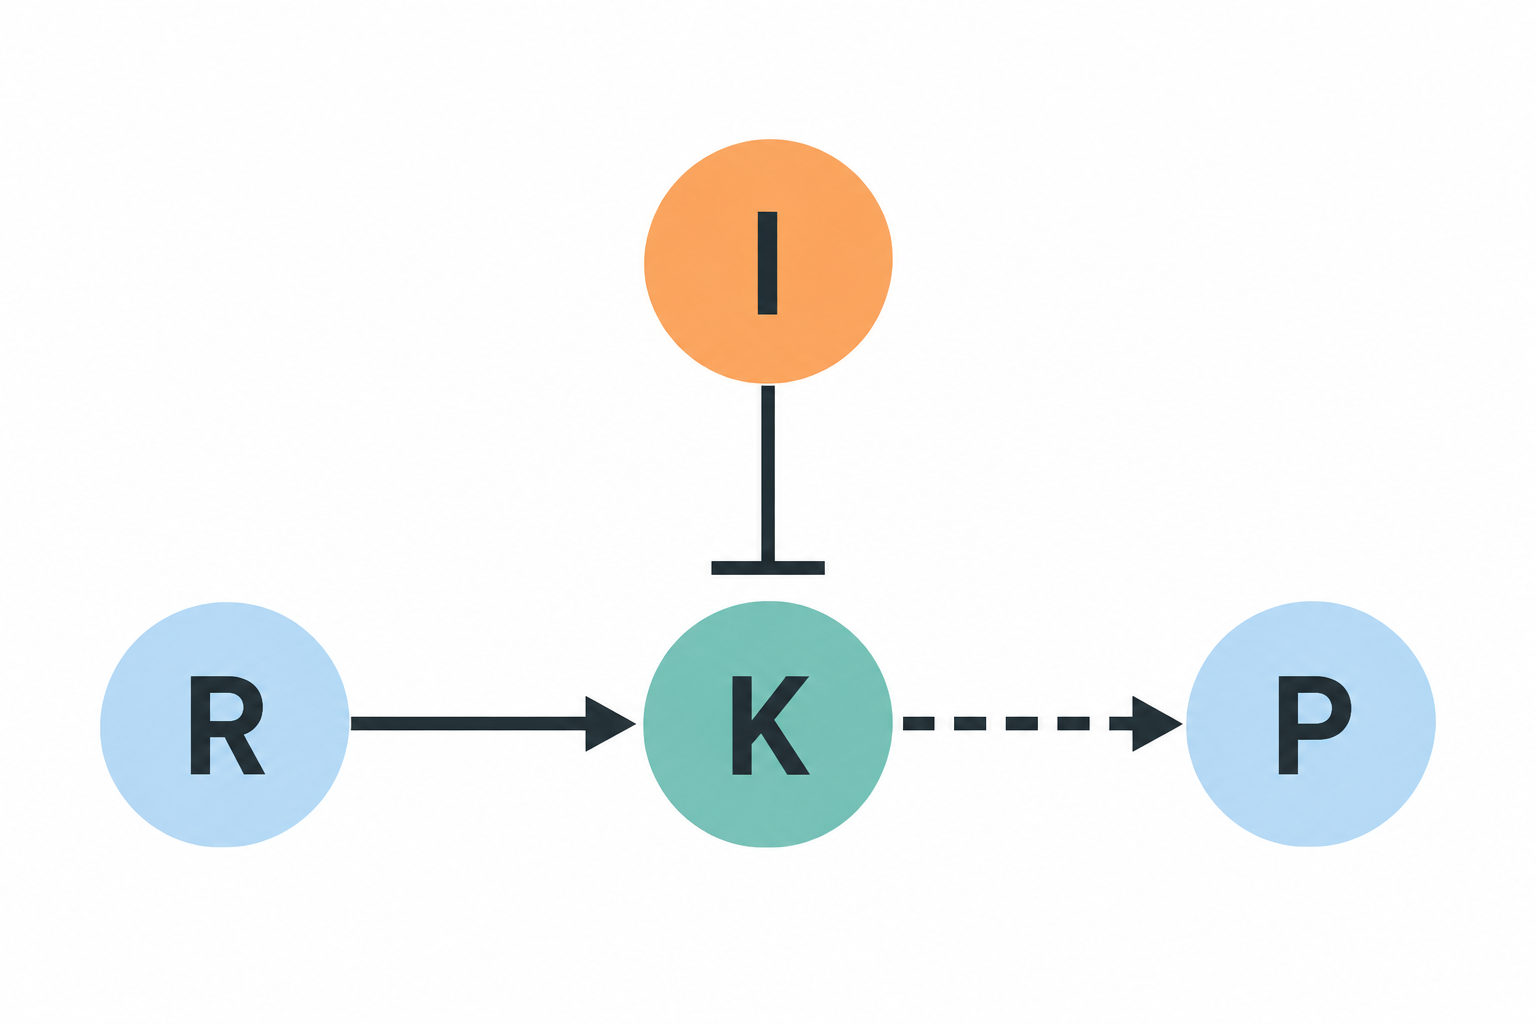
\includegraphics[width=\linewidth]{figures/mechanism-codex.png}
\caption{An actual candidate from Codex's built-in image generation. A solid arrow, dashed arrow, and T-bar express the three stipulated relationships. All four symbols and relationships are fictional. This output was generated in Codex, not in SciDraw AI.}
\label{fig:mechanism}
\end{figure}

Line styles and arrowheads have no universal meaning outside context. Their meaning depends on disciplinary convention, the definitions in the figure, and its legend. The conventions here distinguish three relationships. A real project should use forms its audience understands and add explicit labels where ambiguity remains.

Review the result row by row: locate R and K and inspect the direction; check that the K-to-P connection remains dashed; then confirm that I's inhibitory endpoint is K. “Does this look right?” becomes a set of locatable questions.

\section{Write an executable instruction for the mechanism}

Select the mechanism-and-workflow route in the SciDraw AI guide, replace its default brief, and download a copy.

\begin{Prompt}
[Audience and use] Scientific-figure teaching; no biology background required.
[Purpose] Distinguish given, hypothetical, and inhibitory relationships.
[Source] Only the fictional model specified here.
[Objects] R, K, P, I; each appears once.
[Relationships]
R activates K: a solid arrow from R to K.
K may influence P: a dashed arrow from K to P.
I inhibits K: a line ending with a perpendicular T-bar next to K.
[Layout] R, K, P from left to right; I above K.
[Visual language] White background; simple two-dimensional shapes; identify every object by its letter.
[Constraints] Add no objects, relationships, molecular forms, or experimental results.
[Legend] Explain the three line conventions and identify the fictional teaching model.
[Review] Four objects and three relationships; check direction, endpoints, and labels.
\end{Prompt}

This instruction provides concrete quality criteria: identifiable objects, accurate relationships, and a hypothesis that remains distinguishable from a given relationship. Color can be refined later; the relationships must hold first.

In the mechanism tool, place the instruction in the generation field. Review a candidate against the relationship table before requesting further changes. If an extra object appears, identify it and restate the requirement for exactly four objects, rather than asking only for a simpler design.

For this edition, Codex's built-in image generator produced Figure~\ref{fig:mechanism}. The complete executed prompt and review are included in the repository. The four labels and three relationship types match the brief. Soft tonal variation remains inside the nodes, so this is a checked teaching candidate, not proof that every style constraint was followed exactly. It is not a SciDraw AI output.

The executed generation prompt uses labels alone, with the explanatory words moved to the caption. This is an intentional layout choice recorded in the provenance. Outputs can vary between runs; an instruction does not guarantee that all requirements will be met automatically.

\section{For a data plot, specify constraints by column}

A data brief must connect study design to table structure. Three columns in the first exercise already illustrate several possible ambiguities.

\texttt{sample\_id} identifies an object. \texttt{before} and \texttt{after} contain its two measurements. Eight rows represent eight fictional objects and sixteen observations. State object and measurement counts separately. In real research, also explain experimental units, repeated measurements, and technical replicates.

\begin{Prompt}
Read the uploaded paired-example.csv.
sample_id is the pairing key. before and after are two measurements in a.u.
Create a paired point-and-line plot, with before then after on the x-axis.
Connect the two observations belonging to each object.
Keep all eight objects and the sixteen original values.
Do not treat the columns as independent samples or connect different objects.
Title: "Simulated teaching data: individual changes".
Show the measurements without significance tests or error bars.
Do not remove SIM04 or change its decrease into an increase.
\end{Prompt}

The final line is a check against the file: SIM04 really does decrease from 18 to 17 in this exercise. It does not prescribe a desired finding for real research. Define checks from your actual data, rather than forcing the figure to match an expected conclusion.

“No error bars” is also specific to this exercise. When a different plot needs them, define whether they represent standard deviation, standard error, a confidence interval, or another quantity, and identify how it is calculated. “Add standard error bars” cannot be used as a vague synonym for any uncertainty interval.

\section{When using a PDF helper, establish what was read}

A paper's information is distributed across its abstract, body, figures, methods, and supplementary materials. How text is extracted affects the content available to a visual-prompt helper.

The SciDraw AI PDF helper examined for this edition reads up to the first five pages and uses a limited extract from the abstract or beginning of the document. It can assist with a research overview, but this does not establish that the entire paper, every figure, and the supplements have been interpreted.

Before using it, prepare author-confirmed points: the research question, main method, result to show, and relevant conditions. Compare the helper's prompt with that list, restore omitted information, and only then proceed to drawing. A key result appearing later in a paper may be absent from an input limited to its opening pages.

Record the input scope in the brief. For example: “Author-prepared abstract and result notes; PDF assistance used for drafting; key statements checked against the original.” This is more accurate than “automatically generated from the full paper” and makes future reconstruction easier.

\section{Turn vague feedback into reviewable requests}

Repeated generation can become a search for a more appealing image without a clear purpose. Give each operation a defined job.

\begin{center}\small
\begin{tabularx}{\linewidth}{p{0.25\linewidth}Y}
\toprule
\textbf{Vague feedback} & \textbf{A more concrete request} \\
\midrule
More professional & Align R, K, and P horizontally; use one label size; retain all objects and relationships. \\
Emphasize the result & Make the two measurements directly comparable while retaining individual lines and all observations. \\
Simplify it & Remove decorative backgrounds and repeated explanation; retain four objects, three relationships, and the legend. \\
Journal style & Use a white background and less decoration; apply the agreed text hierarchy and color roles. \\
Complete the legend & Draft what can be identified from the image; the author supplies sample sizes, conditions, and statistical methods. \\
\bottomrule
\end{tabularx}
\end{center}

These requests do not guarantee error-free execution. They make execution assessable. Image edits can affect the whole image, so even a request to change one label should be followed by another check of objects and relationships.

\section{Read the brief as if the research were unfamiliar}

Temporarily set aside the background in your head and look for missing information in the text.

“The treatment group is higher” lacks a variable, condition, and evidential basis. “Split into two groups after this step” lacks a grouping rule. “Improves performance” lacks a metric, unit, and comparison. Supply the missing information or mark the claim as unresolved.

A small mapping table can help: statement, source location, visual representation, and question still to resolve. In real projects, identify a column, file version, or record page. In this exercise, identify a teaching assumption. This prevents poorly sourced claims from slipping into an image.

\section{Exercise and acceptance criteria}

Complete two briefs: one for your research and one for either the fictional mechanism or paired-data example. Retain the original description and write a short revision note explaining which relationships, sources, and acceptance criteria you added.

Check whether objects can be counted, relationships can be examined one by one, data constraints map to columns, unknowns remain explicit, and the output has a concrete use.

You now have an input that can move into figure creation. Chapter 3 will explore different compositions from the same brief and compare the work they ask the reader to do.
